\documentclass[svgnames]{article}
\usepackage[utf8]{inputenc}
\usepackage{amsmath}
\usepackage{amssymb}
\usepackage{mathrsfs}
\usepackage{mathtools}
\newtheorem{mydef}{Given}
\newtheorem{mytheorem}{Theorem}
\usepackage{enumitem}
\usepackage{venndiagram}
\usepackage{smartdiagram}
\usepackage{caption}
\usepackage{subcaption}
%\usepackage[framed,numbered,autolinebreaks,useliterate]{mcode}
\usepackage{pgfplots}
%\usepackage{tkiz}
\usepackage{listings}
\definecolor{dkgreen}{rgb}{0,0.6,0}
\definecolor{gray}{rgb}{0.5,0.5,0.5}
\definecolor{mauve}{rgb}{0.58,0,0.82}
\usepackage{float}

\lstset{ %
  language=R,                     % the language of the code
  basicstyle=\footnotesize,       % the size of the fonts that are used for the code
  numbers=left,                   % where to put the line-numbers
  numberstyle=\tiny\color{gray},  % the style that is used for the line-numbers
  stepnumber=1,                   % the step between two line-numbers. If it's 1, each line
                                  % will be numbered
  numbersep=5pt,                  % how far the line-numbers are from the code
  backgroundcolor=\color{white},  % choose the background color. You must add \usepackage{color}
  showspaces=false,               % show spaces adding particular underscores
  showstringspaces=false,         % underline spaces within strings
  showtabs=false,                 % show tabs within strings adding particular underscores
  frame=single,                   % adds a frame around the code
  rulecolor=\color{black},        % if not set, the frame-color may be changed on line-breaks within not-black text (e.g. commens (green here))
  tabsize=2,                      % sets default tabsize to 2 spaces
  captionpos=b,                   % sets the caption-position to bottom
  breaklines=true,                % sets automatic line breaking
  breakatwhitespace=false,        % sets if automatic breaks should only happen at whitespace
  title=\lstname,                 % show the filename of files included with \lstinputlisting;
                                  % also try caption instead of title
  keywordstyle=\color{blue},      % keyword style
  commentstyle=\color{dkgreen},   % comment style
  stringstyle=\color{mauve},      % string literal style
  escapeinside={\%*}{*)},         % if you want to add a comment within your code
  morekeywords={*,...}            % if you want to add more keywords to the set
} 


%\renewcommand{\theenumi}{\Alph{enumi}}
\newenvironment{amatrix}[1]{%
  \left(\begin{array}{@{}*{#1}{c}|c@{}}
}{%
  \end{array}\right)
}

\newenvironment{tolerant}[1]{%
  \par\tolerance=#1\relax
}{%
  \par
}


\pgfmathdeclarefunction{gauss}{2}{%
  \pgfmathparse{1/(#2*sqrt(2*pi))*exp(-((x-#1)^2)/(2*#2^2))}%
}


\title{Statistical Methods: Final}
\author{Cameron McIntyre}
\date{\today}

\begin{document}

\maketitle

\section*{1}
A new treatment was advertised to reduce the incidence of a common illness. It was possible to get the illness more than once. Consider 500 individuals who participated in an experiment and were randomly assigned to treatment and placebo groups. Test the null hypothesis that the treatment and placebo populations are equivalent.

\begin{center}
\begin{tabular}{| c | c | c | c |} 
\hline
& No contractions & 1 contraction & $>$ 1 contraction \\
\hline
Treatment & 252 & 145 & 103 \\
\hline
Placebo & 224 & 136 & 140 \\
\hline
\end{tabular}
\end{center}

\subsection*{Answer:}

We use a chi square goodness of fit test. 
$H_0$: The treatment group fits the data well based on the proportions estimated by the placebo group.
\newline
$H_1$: The treatment group does not fit the data well based on the proportions estimated by the placebo group
\newline

We estimate proportions:
$$P(No\ contractions) = \frac{224}{500}=.448$$
$$P(1\ contractions) = \frac{136}{500}=.272$$
$$P(>1\ contractions) = \frac{140}{500}=.28$$

We form our test statistic:

$$\sum^{3}_{1} \frac{(O-E)^2}{E}=\frac{(252-.448*500)^2}{.448*500}+\frac{(145-.272*500)^2}{.272*500}+\frac{(103-.28*500)^2}{.28*500}$$
$$\sum^{3}_{1} \frac{(O-E)^2}{E}=\frac{(252-224)^2}{224}+\frac{(145-136)^2}{136}+\frac{(103-140)^2}{140}$$
$$\sum^{3}_{1} \frac{(O-E)^2}{E}=\frac{784}{224}+\frac{81}{136}+\frac{1369}{140}$$
$$\sum^{3}_{1} \frac{(O-E)^2}{E}=3.5 + 0.595+ 9.778= 13.874$$

Now using the chi - square distribution $\chi_{.95, 2}= 5.991465$.

Since $13.874>5.9914$, we reject $H_0$ and conclude that the populations are not equivalent. 

\section*{2}
Consider two competing manufacturers in the production of a component for a system. The nominal specification is 15 mm, and both manufacturers may meet that spec. However, there is question about the variability of for each. Test the hypothesis that $H_0: \sigma_X^2 = \sigma_Y^2$ versus $H_a: \sigma_X^2 \neq \sigma_Y^2$ assuming the data are from normal distributions.

\begin{center}
\begin{tabular}{c c} 
\hline
X & Y \\
\hline
   26.37 &  18.67 \\
    8.75 &  16.55\\
   13.68 & 16.35\\
   14.39 &  17.12\\
    6.94 &  14.50\\
   18.92 &  13.00\\
   14.67 &  17.55\\
   15.78 &  17.07\\
   20.98 &  13.27\\
   14.39 &  16.18\\
   \hline
\end{tabular}
\end{center}

\subsection*{Answer:}
$$H_0: \sigma^2_x = \sigma^2_y $$
$$H_1:\sigma^2_x \neq \sigma^2_y $$
We will use an F test:
$$S_x= \frac{n\sum x_i^2 - (\sum x)^2}{n(n-1)}=\frac{10*2683.7337 - (154.87)^2}{90}=31.69$$
$$S_y= \frac{n\sum y_i^2 - (\sum y)^2}{n(n-1)}=\frac{10* 2599.411 - (160.26)^2}{90}=3.45$$

Our test statistic is the ratio of the two sample Variances. 
$$\hat{F} = \frac{S_x}{S_y}=\frac{31.69}{3.45}=9.177$$

Now $\frac{S_x}{S_y}\sim F_{n-1,m-1}$, So our critical values are $F_{.025,9,9}=0.2483859$ and $F_{.975,9,9}=4.025994$.
\newline
Since $9.177>4.025994$, we reject $H_0$ and infer the variances are not the same.

\section*{3}
Let $f_X(x) = 1/\theta X^{(1-\theta)/\theta}, 0 < x <1$. 

\begin{enumerate}[label=\roman*.]
\item Find the MLE for $\theta$. 
\item Determine whether or not the estimator is unbiased.
\end{enumerate}

\subsection*{Answer:}

\begin{enumerate}[label=\roman*.]
\item Find the MLE for $\theta$. 

$$L(\theta, x) = \big( \frac{1}{\theta}\big)^n \Pi x_i^{\frac{1}{\theta}-1} $$
$$log(L(\theta, x))= n \frac{1}{\theta} + (\frac{1}{\theta}-1)log(\Pi x_i)$$
$$\frac{d}{d\theta}log(L(\theta, x)) = -\frac{n}{\theta} -\frac{1}{\theta^2}log(\Pi x_i)$$
We set this to 0.

$$0 = -\frac{n}{\theta} -\frac{1}{\theta^2}ln(\Pi x_i) \leftrightarrow  \hat{\theta}_{MLE} = \frac{\sum ln( x_i)}{-n}$$
Note, $0<y_i<1$, therefore $ln(y_i)< 0$ and $\hat{\theta}>0$
\item Determine whether or not the estimator is unbiased.

The estimate is unbiased.
$$E[\hat{\theta}] =E[\frac{\sum ln( x_i)}{-n}]=\int_{0}^{1}-\frac{n ln(x)}{n}\frac{1}{\theta}x^{\frac{(1-\theta)}{\theta}}dx$$
Let $u=x^{\frac{1}{\theta}}dx$ then, $d(x^{\frac{1}{\theta}})= \frac{1}{\theta}x^{\frac{1}{\theta}-1}dx$, therefore.
$$E[\hat{\theta}] = -\int^{1}_{0}ln(x)d(x^{\frac{1}{\theta}})= -[x^{\frac{1}{\theta}}ln(x)\bar|^{1}_{0} - \int_{0}^{1}x^{\frac{1}{\theta}-1}]$$
$Lim_{x ->0}x^{\frac{1}{\theta}}ln(x)=0$ for $\theta>0$ So,
$$E[\hat{\theta}]=\int_{0}^{1}x^{\frac{1}{\theta}-1}=\theta x^{\frac{1}{\theta}}\bar|^{1}_{0}=\theta - lim_{x->0}\theta x^{\frac{1}{\theta}}=\theta-0=\theta$$
So $E[\hat{\theta}]=\theta$.
\end{enumerate}

\section*{4}
Consider the density $f_X(x) = (1-p)^x p, x= 0, 1, ...$ and a random sample from that distribution of ${3, 34, 7, 4, 19, 2, 1, 19, 43, 2, 22, 4, 19, 11, 7, 1, 2, 21, 15, 16}$. Determine the method of moments estimator for $p$ and estimate its value using the random sample.

\subsection*{Answer:}
Method of moments.
$$\mu= \sum_{x=0}^1x p(1-p^x) = \frac{1}{p}$$
Equating $\bar{x}$ to the first moment.
$$\mu=\bar{x} \leftrightarrow \frac{1}{p} = \bar{x} \leftrightarrow \hat{p}= \frac{1}{\bar{x}}$$

Now we estimate p.

$$\hat{p}=\frac{1}{\frac{3 + 34 + 7 + 4 +19 + 2 + 1 + 19+ 43+  2, 22+  4+ 19+ 11+ 7+  1+ 2+ 21+  15+  16}{20}} = \frac{1}{12.6}=0.0793$$

\section*{5}
The number of students coming for treatment at a health facility each half hour was recorded: $\{3, 3, 2, 0, 4, 5, 6, 4, 4, 3, 2, 1, 2, 3, 0, 5, 5, 3, 2, 3, 5, 4, 1, 2, 0, 3, 2, 4, 2, 6\}$. Do these data follow a Poisson distribution? Conduct the appropriate Chi-Square test.

\subsection*{Answer:}

We use the unbiased estimate for $\lambda = \bar{X}$.

$$\bar{X} = \frac{\sum x_i}{n} = \frac{89}{30} = 2.966$$


We use a Chi Square Goodness of fit test.
\newline
$H_0:$ The data fits a poisson distribution well.
\newline
$H_1:$ The does not fit a poisson distribution well.
We form our test statistic.
$$\chi^2_{29} = \sum { \frac{(X-\lambda)^2}{\lambda}} = \frac{80.9666}{3}=27.29213$$

Using R we find our critical value of 42.55.
Therefore we do not reject $H_0$ And the data does follow a poisson distribution. 
\begin{lstlisting}
> qchisq(.95,29)
[1] 42.55697
> pchisq(26.988, 29)
[1] 0.4276474
\end{lstlisting}

\section*{6}
Suppose an airport metal detector catches a person with metal 99\% of the time. That is, it misses detecting a person with metal 1\% of the time. Assume independence of people carrying metal. What is the probability that less than a plane full carrying metal, 200, coming through the metal detector would be needed to miss three?

\subsection*{Answer:}
The distribution of the failures to detect a person with metal can be considered to be Negative Binomial with parameter $p=.01$. We want to see the number of trial being less than 200 for three failures. 
\newline
Since the number of trials is very large (200), we will invoke the central limit theorem and approximate this using the Demoivre Laplace theorem.

\fbox{\begin{minipage}{30em}
\textbf{Theorem 4.32}
(DeMoivre-Laplace) Let X be a binomial random variable defined on n independent trials for which $p=P(success)$. For any numbers a and b


$$lim_{n->\infty}P(a<\frac{x-np}{\sqrt{np(1-p}}<b)=\frac{1}{\sqrt{2\pi}}\int^{a}_{b}e^{\frac{z^2}{2}}dz$$

\end{minipage}}

$$E[X] =\frac{r}{p}=\frac{3}{.01} = 300$$ 
$$Var[X] = \sqrt{\frac{r(1-p)}{p^2}}=\sqrt{\frac{3(.99)}{.01^2}}=172.3369$$

We need to add the \textbf{continuity correction} (because we are going from a discrete to a continuous distribution, and take the probability over the support for the pmf. Note that the negative binomial distribution is only defined over the support of $X>r$ where r is the number of successes - Therefore we add the adjustment of $E[X] =\frac{r}{p} - r = 297$

$$P(X<200 | Succeses = 3) = P(X <200.5)$$
$$=P(X< \frac{200.5- (\frac{3}{.01} -3) }{\sqrt{\frac{3(.99)}{.01^2}}})= Z(-0.5773605)$$
$$P(X<200)=0.2877569$$

Therefore the probability is 28.77 \%.

\section*{7}
The tensile strength of a fiber, in pounds per square inch, has a mean $\mu = 40$ and standard deviation $\sigma = 4$. A random sample of $n= 120$ is taken from a distribution of tensile strengths. Compute the probability that the sample mean $\bar{x}$ exceeds 39.3 pounds per square inch?

\subsection*{Answer:}

The distribution is approximately $\bar{X} \sim N(40, \frac{4}{\sqrt{120}})$
So,

$$P(\bar{x}>39.3) = P(z> \frac{39.3-40}{ \frac{4}{\sqrt{120}}})$$
Where $z\sim N(0,1)$.
\newline
Using R.
\begin{lstlisting}
> 1-pnorm(39.3, mean=40, sd = 4/sqrt(120))
[1] 0.9723829
\end{lstlisting}
So  $P(\bar{x}>39.3) =  0.9723$

\section*{8}
Consider the density:
$$f_{x}(x)=\frac{1}{\Gamma(\alpha)\theta^{\alpha}}x^{\alpha-1}e^\frac{x}{\theta}, 0\leq x < \infty$$
for the random variable X. Suppose a random sample $X_1,X_2,....X_n$ is taken. Using this random sample, develop a
sufficient statistic for the parameter $\theta$.

\subsection*{Answer:}
We consider the likelihood function of this distribution. 
$$L_p(x:\theta)=\Pi_{i=1}^{n}\frac{1}{\Gamma(\alpha)\theta^{\alpha}}x^{\alpha-1}e^\frac{x}{\theta}$$
$$L_p(x:\theta)=\Big(\frac{1}{\Gamma(\alpha)\theta^{\alpha}}\Big)^n \Pi_{i=1}^n x_i^{\alpha-1}e^{\frac{1}{\theta}\sum x_i}$$

We know by the factorization theorem that $\hat{\theta}$ is a sufficient statistic for  $\theta$  if and only if we can find a factorization $L_p = g(h(X), \theta)d(X)$ Where $X$ is a vector from the distribution. 
\newline
We re organize the statement above.
$$L_p(x:\theta)=\Big(\frac{1}{\Gamma(\alpha)\theta^{\alpha}}\Big)^n e^{\frac{1}{\theta}\sum x_i} \Pi_{i=1}^n x_i^{\alpha-1}$$
We see that 
$$g(h(X), \theta) = \Big(\frac{1}{\Gamma(\alpha)\theta^{\alpha}}\Big)^n e^{\frac{1}{\theta}\sum x_i} $$
And,
$$d(X) = \Pi_{i=1}^n x_i^{\alpha-1}$$

Therefore $\sum_{i=1}^{n}x_i$ is a sufficient statistic for $\theta$. 

\section*{9}
Let $X_1,X_2,....X_8$ be a random sample of size n = 8 from a Poisson distribution with mean $\lambda$.
Reject the null hypothesis $H_0: \mu= 0.5$ in favour of $H_a: \mu > 0.5$ if the observed sum $\sum_{1}^{8}x_i \geq 8$. Construct a power function for the test, clearly indicating the significance level $\alpha$ for the test.

\subsection*{Answer:}
The sum of 8 poisson random variables is a poisson random variable with parameter $\lambda_{sum} = 8* \lambda$. Under the null hypothesis $\lambda_{sum} = 8* \lambda = 8*.5=4$. We reject when $\sum_{1}^{8}x_i \geq 8$. This means the alpha of the test is 
$$\alpha = 1- \sum_{i=0}^{7}\frac{1}{e^{4}}\frac{4^i}{i!}=1-0.9488664=0.05113362$$

The power of the test is the probability we reject $H_0$ for a given rejection criteria (in this case $\sum_{1}^{8}x_i \geq 8$) and a specified value for $\lambda$.
\newline
Our expression for the power is:
$$1-\beta=P(reject\ H_0 | \lambda = \tilde{\lambda}) = 1 - P(\sum X_i < 8 | \lambda = \tilde{\lambda})) = 1- \sum_{i=0}^{7}\frac{1}{e^{\tilde{\lambda}}}\frac{\tilde{\lambda^i}}{i!}$$

We plot this expression below. 
\begin{lstlisting}
1-ppois(7, (1:20))
plot((1:20)/8, 1-ppois(7, (1:20)), xlab = 'Values for Lambda', ylab = "Power of the test")
\end{lstlisting}
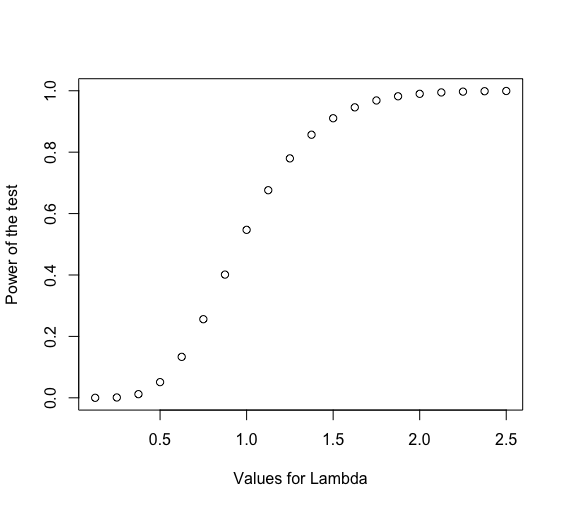
\includegraphics[scale=.5]{powercurve}

\begin{center}
\begin{tabular}{| c | c |} 
\hline
Lambda & Power of Test\\
\hline
 0.125&0.0000102492\\
0.25&0.001096719\\
0.375&0.0119045039\\
0.5&0.0511336158\\
0.625&0.1333716741\\
0.75&0.2560202395\\
0.875&0.4012861645\\
1&0.5470391905\\
1.125&0.6761030357\\
1.25&0.7797793534\\
1.375&0.8568084653\\
1.5&0.9104955032\\
1.625&0.9459717516\\
1.75&0.9683803444\\
1.875&0.9819978069\\
2&0.990000219\\
2.125&0.9945669808\\
2.25&0.9971065349\\
2.375&0.9984866574\\
2.5&0.9992214099\\
\hline
\end{tabular}
\end{center}


\section*{10}
A recurring problem in the field required several hours to fix. A new approach is intended to speed the repair. Assuming the variances may be assumed equal and that repair data is approximately normal, conduct a two-sample test  $H_0: \mu_{old} = \mu_{new}$ vs $H_0: \mu_{old} > \mu_{new}$using the data below. Report the p-value of the test.


$$Old = 4.3, 6.5, 4.6, 4.3, 6.4, 4.8, 5.1, 6.8, 4.9, 4.5, 5.1, 7.3, 3.3, 5.0, 4.6, 7.0, 5.1, 3.8, 5.2, 4.1, 5.7$$

$$New = 6.2, 4.0, 3.3, 4.5, 2.3, 3.0, 3.2, 6.0, 3.7 4.5, 5.3, 4.0, 5.4, 4.3, 3.8$$

\subsection*{Answer:}
$H_0: \mu_{old}=\mu_{new}$
\newline
$H_1: \mu_{old} \neq \mu_{new}$

$$\mu_{old} = 5.161$$
$$\mu_{new} = 4.233$$

$$S^2_{pooled}=\frac{(n-1)S_{old}^2+(m-1)S_{new}^2}{n+m-2}=\frac{(20)S_{old}^2+(14)S_{new}^2}{34}=1.13$$

$$T_{33}=\frac{5.161-4.233}{1.096\sqrt{\frac{1}{21}+\frac{1}{15}}}=2.504$$

$$T_{.95, 34}= 1.690924$$

Since our test statistic $2.504> T_{.95, 34}$, We reject the null hypothesis and conclude that the old method had a higher mean service time than the new method.


\section*{11}
 A clue to the amount of organic waste in a lake was the number of bacteria colonies in 100 millilitres of water. The number of colonies, in hundreds, for $N = 30$ samples of water from one portion of the lake yielded.
 
 $$93, 140, 8, 120, 3, 120, 33, 70, 91, 61, 7, 100, 19, 98, 110$$
$$23, 14, 94, 57, 9, 66, 53, 28, 76, 58, 9, 73, 49, 37, 92$$

Construct an approximate 95\% confidence interval for the mean number $\mu$ of colonies in 100
millilitres of water in this portion of the lake.
\subsection*{Answer:}
$\mu = 60.36667$
\newline
$S_x = 39.62191$
\newline

$\bar{X} \sim N(60.36667, 39.62191^2)$

$$P(60.36667 - 1.96 * \frac{39.62191}{\sqrt{30}}< \bar{X} <60.36667 + 1.96 * \frac{39.62191}{\sqrt{30}})=.95$$
$$P(46.62219< \bar{X} < 74.11115 )=.95$$
So our confidence interval is.

$$[46.62219, 74.11115 ]$$

\section*{12}
In enzyme kinetics for a type of reversible reactions, the Michaelis-Menton equation relates the velocity of the reaction to the concentration of the substrate through the model:
$$ v = \frac{v_{max}[S]}{K_m + [S]}$$
where $v$ is the reaction velocity, $V_{max}$ is the maximum velocity for the reaction saturated with substrate, $[S]$ is the concentration of the substrate, and $K_m$ is the Michaelis constant, representing the concentration where the reaction is$ \frac{1}{2} V_{max}$.

$$ S =  0.998, 0.996, 0.952, 0.944, 0.923, 0.904, 0.921, 0.909, 0.869, 0.874, 0.881$$
$$ 0.838, 0.834, 0.844, 0.781, 0.805, 0.823, 0.808, 0.774, 0.745, 0.747$$
$$ V = 125.000, 100.000, 50.000, 33.333, 25.000, 20.000, 16.667, 14.286, 12.500,$$
$$11.111,10.000, 9.091, 8.333, 7.692, 7.143,6.667, 6.250, 5.882, 5.556, 5.263, 5.000$$

Determine the regression model that will provide estimates of $\frac{k_m}{V_{max}}$  and  $\frac{1}{V_{max}}$; and provide a 95\% confidence interval for each.
\subsection*{Answer:}

We take the reciprocal of the equation. 
$$\frac{1}{v} = \frac{v_{max}}{K_m}\frac{1}{S} + \frac{1}{V_{max}}$$

We can take this as a linear model of the form $\hat{y} = \beta_0 + \beta_1X$ where $\hat{y} = \frac{1}{v}$, $ \beta_0 =  \frac{1}{V_{max}}$,  $\beta_1=  \frac{v_{max}}{K_m}$. and $X=\frac{1}{S}$

We have our estimates of $\hat{\beta_1}$ and $\hat{\beta_0}$.

$$\hat{\beta_1} = \frac{n\sum x_i Y_i - (\sum x_i)(Y_i)}{n(\sum x_i^2) - (\sum x_i)^2} =  \frac{21 *2.575092 - 24.44674*2.107999}{n(\sum x_i^2)}  = \frac{21*2.57-24.4*2.10}{21*597.64 - 24.44} = 0.5877836$$
$$\hat{\beta_0} = \bar{Y} - \hat{\beta_1}\bar{x}= 0.1003809 - 0.6842569 = -0.583876 $$

So our estimate for $\frac{k_m}{V_{max}}$  is $\hat{\beta_1} = -0.5877836$, and our estimate for $\frac{1}{V_{max}}$ is $\hat{\beta_0} = -0.583876 $ \newline 

Our $95\%$ confidence interval for  $\frac{k_m}{V_{max}} = \hat{\beta_1}$
$$[\hat{\beta_1} - t_{\frac{.05}{2},19}\frac{s}{\sqrt{\sum(x-\bar{x})^2}}, \hat{\beta_1}  + t_{\frac{.05}{2},19}\frac{s}{\sqrt{\sum(x-\bar{x})^2}}]$$
$$[ 0.58778  -2.093024 \frac{0.01500231}{0.4539154},  0.58778+ 2.093024 * \frac{0.01500231}{0.4539154}]$$
$$[0.5186037,0.6569563]$$

Our $95\%$ confidence interval for  $\frac{1}{V_{max}} = \hat{\beta_0}$
$$[\hat{\beta_0} - t_{\frac{.05}{2},19}\frac{s\sqrt{\sum x_i^2}} {\sqrt{n}\sqrt{\sum(x-\bar{x})^2}},\hat{\beta_0} + t_{\frac{.05}{2},19}\frac{s\sqrt{\sum x_i^2}} {\sqrt{n}\sqrt{\sum(x-\bar{x})^2}} ]$$
$$[-0.583876 - 0.001274822, -0.583876 + 0.001274822]$$
$$[-0.5851508, -0.5826012]$$

\section*{13}
 A dart target 24" in diameter is marked in five concentric circular bands (point values 10, 20, 40, 60, 80), which are 2" in width and a centre bullseye circle (point value 100), which is 4" in diameter. A blindfolded dart thrower is randomly tossing darts at the target and the point values of the darts are totalled. Suppose 5 hit the target randomly. What is the probability the thrower scores 140 in the 5 tosses?

\subsection*{Answer:}
We start by figuring out the probabilities:

$$P(X=10) = \frac{\pi (12^2-10^2)}{\pi 12^2} = \frac{44}{144} = 0.3055$$
$$P(X=20) = \frac{\pi (10^2-8^2)}{\pi 12^2} = \frac{36}{144} = 0.25$$
$$P(X=40) = \frac{\pi (8^2-6^2)}{\pi 12^2} = \frac{28}{144} = 0.194$$
$$P(X=60) = \frac{\pi (6^2-4^2)}{\pi 12^2} = \frac{20}{144} = 0.1388$$
$$P(X=80) = \frac{\pi (4^2-2^2)}{\pi 12^2} = \frac{12}{144} = 0.083$$
$$P(X=100) = \frac{\pi 2^2}{\pi 12^2} = \frac{4}{144} = 0.0277$$

$$P(\sum X=140) =  \frac{5!}{3!2!}0.194^3 0.3055^2+ \frac{5!}{3!2!}0.25^3 0.194^2 + \frac{5!}{1!1!1!2!}0.1388^1 0.194^1 0.25^1 .3055^2$$% 60  40  1 20 2 10 
$$+ \frac{5!}{1!4!}0.1388^1 0.25^4 + \frac{5!}{1!2!2!}0.083^1 0.25^2 0.3055^2 +\frac{5}{1!4!}0.0277^1 0.3055^4$$ %100 4 10

$$P(\sum X=140) = .0012107 + .014588 + .037821 + .002713 + .006864 + .005908$$
$$P(\sum X=140) = .0691$$

\section*{14}
A true regression model of $Y_i = \beta_0+\beta_1X + \epsilon_i $ has as its parameters $ \beta_0 = 50$ and $ \beta_1 = 20$ 
when the response is fit to the designed X values 10, 20, 30, 40, 50, 60, 70, 80, 90, and 100, each time with 2 observations taken for each X. The variance, $\sigma_y^2 = 4$. Simulate the slope coefficient $\beta_1$ by randomly sampling 20 observations for $Y_i$ according to this design and computing the slope estimate $b_1$. Repeat this simulation 100 times. 
\begin{enumerate}
\item 
Rank the values for $b_1$ and report the 20th and 80th quantile. 
\item
For one additional simulation, take the values (x, y), and fit the model experimentally, and compute the 80\% confidence interval for $\beta_1$. Briefly, discuss the agreement/disagreement of the simulated interval quantiles and the confidence interval.
\end{enumerate}
\subsection*{Answer:}
\begin{enumerate}
\item 
We know for a Linear Model:
$$Y_i = E[Y|x] = \beta_0+\beta_1 x$$
And also as a property of the linear model,The standard deviation, $\sigma$, associated with $f_{Y|x}(y)$ is the same for all x.
So,
$$\sigma^2_y = 4 $$
So $E[Y|x] = \beta_0+\beta_1 x$ and $\sigma^2_y=4$. In our simulation code, we define this simulation of $Y_i\sim N( 50 +20 x,2^2)$ and the transformation $\beta_1 = \frac{Y-\beta_0}{\bar{x}}$ to get our estimates for $b_1$.
\begin{lstlisting}
> X_VALS <- c(10, 20, 30, 40, 50, 60, 70, 80, 90, 100,10, 20, 30, 40, 50, 60, 70, 80, 90,100)
>
> ret_b_estimate <- function(a,b) {
+   return((a-50)/b)
+ }
> 
> 
> b_estimates <- c()
> for (i in (1:100)){
+   x_samp = sample(X_VALS, 20, replace = TRUE)
+   x_samp1 = 20*x_samp +50
+   y_simulate = rnorm(20, x_samp1, sd = 2)
+   b_estimates = c(b_estimates, ret_b_estimate(y_simulate,x_samp))
+ }
> 
> sort(b_estimates)[2000*.2]
[1] 19.96522
> sort(b_estimates)[2000*.8]
[1] 20.03319
\end{lstlisting}
So our estimates for the $20^{th}$ quantile is 19.96522 and the $80^{th}$ quantile is 20.03319.
\item

We simuate more values for $Y_i$ and we calculate  $\beta_1= \frac{n\sum x_iy_i - \sum x_i \sum y_i}{n(\sum x_i^2)- (\sum x_i)^2)}=20.00942$, $\beta_0=\bar{y}- \hat{\beta_1}\hat{x}=49.06816$:
\begin{lstlisting}
X_VALS <- c(10, 20, 30, 40, 50, 60, 70, 80, 90, 100,10, 20, 30, 40, 50, 60, 70, 80, 90,100)

x_samp = sample(X_VALS, 20, replace = TRUE)
y_samp1 = 20*x_samp +50
y_simulate = rnorm(20, y_samp1, sd = 2)

b_1 = (20*sum(x_samp*y_simulate) - (sum(x_samp)*sum(y_simulate)))/(20*sum(x_samp*x_samp)-sum(x_samp)*sum(x_samp))
b_0 = mean(y_simulate) - b_1 * mean(x_samp)
> b_0
[1] 49.06816
> b_1
[1] 20.00942
> 
s = 1/18*(sum(y_simulate*y_simulate) - b_0*sum(y_simulate) -b_1* sum(x_samp*y_simulate))
> s
[1] 3.483129
> sqrt(sum((x_samp-mean(x_samp))^2))
[1] 151.921
> qt(.2,18)
[1] -0.8620487
> qt(.8,18)
[1] 0.8620487
\end{lstlisting}
We define the confidence interval for $\beta_1$ as follows:
$$\Big[ \hat{\beta_1} - t_{\frac{\alpha}{2},n-2} \frac{s}{\sqrt{\sum(x-\bar{x})^2}}, \hat{\beta_1} + t_{\frac{\alpha}{2},n-2} \frac{s}{\sqrt{\sum(x-\bar{x})^2}} \Big]$$
$$\Big[20.00942 - 0.8620487 \frac{3.483129}{151.921},  20.00942 + 0.8620487 \frac{3.483129}{151.921} \Big]$$
$$\Big[19.98966,20.02918]$$
\end{enumerate}

The estimates versus the quantiles are really quite close. $19.96522, 20.03319$ (simulations) versus $\Big[19.98966,20.02918\Big]$ (confidence interval). We could attribute some of the difference between the simulation to the confidence interval due to the number of simulations. For the simulation answer we were looking at a population of 2000 samples whereas for the confidence interval we looked at one simulation of 20 samples. 


\textbf{EXTRA QUESTIONS FROM THE LAST FINAL THAT WAS POSTED ON BLACKBOARD IN ERROR}

\section*{1}
Let $f(x)=\frac{1}{a}, 0\leq x \leq a$. Derive the method of moments estimator for a based on the random sample of n values from the distribution. Show that this estimator is unbiased or asymptotically unbiased.
\subsection*{Answer:}
$$\frac{\sum_{i=1}^{n} x_i}{n}=\bar{x}=E[x]=\int_{0}^{a}\frac{x}{a}=\frac{x^2}{2a} \Big|^{a}_{0}=\frac{a}{2}$$
$$\leftrightarrow$$
$$2*\bar{x}=\hat{a}$$

Now finding the bias:
$$E[\hat{a}]=E[2*\bar{x}]=E[2*\bar{x}]=2\frac{1}{n}*nE[x]= 2\frac{1}{n}*n\frac{a}{2}= a$$

So the estimator for a is unbiased by the method of moments. 

\section*{2}
Let $f(x)=\frac{1}{a}, 0\leq x \leq a$. Derive the maximum likelihood estimate for a based on the random sample of n values from the distribution. Show that this estimator is unbiased or asymptotically unbiased.
\subsection*{Answer:}

$$L(a|x)=\Pi^{n}_{1}\frac{1}{a}=(\frac{1}{a})^n$$
Taking derivative and maximizing.
$$\frac{d}{dx}L(a|x)=n(\frac{1}{a})^{n-1}, $$
We set to 0
$$0=n{\frac{1}{a}}^{n-1},  0\leq x \leq a$$

We take the limit, as the solution isn't algebraically obvious. 
$$lim_{x\rightarrow \infty}n(\frac{1}{x})^{n-1}=0$$
Therefore the M.L.E is $X_{max}$
To find the bias we need to know the distribution of $X_max$ This is an order statistic so we use the distribution.

$$X_{max}\sim n  * \frac{x^{n-1}}{a^{n}}$$
$$\leftrightarrow$$
$$E[X_{max}]= \int_{0}^{a}n x \frac{x^{n-1}}{a^n} =\int_{0}^{a} n( {\frac{x}{a}})^n$$
$$E[X_{max}]=\frac{n}{(n+1)a^n}x^{n+1}\big|^{a}_{0}=\frac{n}{n+1}a $$
Note, $\frac{n}{n+1}\hat{a}<a$ Therefore this estimate is biased and underestimates a.
As n tends to infinity then $\frac{n}{n+1}\hat{a}\rightarrow a$ and it converges asymptotically. 

\section*{3}
\textbf{NOT COMPLETED }
Adjust the estimators in 1 and 2, if necessary, so they are both unbiased. Report the relative efficiency of the unbiased version of the estimator in 1 to the unbiased version of the estimator in 2.


\subsection*{Answer:}
We adjust the estimator in 2 to make it unbiased. 
\newline
The new estimator for 2 is $\hat{a} = \frac{n+1}{n}X_{max}$. Then $E[\hat{a}]= E[\frac{n+1}{n}X_{max}] = a$, by the linearity of the expectation operator. 



\begin{lstlisting}
shoshani <- c( 0.693,0.662, 0.690, 0.606, 0.570,0.749, 0.672, 0.628, 0.609, 0.844, 0.654, 0.615, 0.668, 0.601, 0.576, 0.670, 0.606, 0.611, 0.553, 0.933)
> med <- sum(shoshani>.618)
> count <- length(shoshani)
> testst <- (med-count/2)/(sqrt(20/4))
> pval <- pnorm(testst)
> med
[1] 11
> count
[1] 20
> testst
[1] 0.4472136
> pval
[1] 0.6726396
> \end{lstlisting}

Since the p value is .67, we fail to reject $H_0$ and conclude that the the rectangles are similar to the golden ratio variety.
\end{document}


\end{document}
